%# -*- coding: utf-8-unix -*-
%%==================================================
\chapter{文字识别(Scene Text Recognition)}
\cite{scatter,2020srn,wan2019textscanner}
\section{文字识别方法介绍}
\subsection{TextScanner}
vhefbhv
\subsection{SCATTER}
\subsection{SRN}
SRN的主要出发点是:
1)在文字识别中,由于光照,旋转等因素的影响,仅仅依靠图像的视觉特征
极易引起单词中某个字符预测错误。对于这些易错的字符,如果能够利用单词的语义信息,那么
将会极大地降低该字符的预测错误率。如图\ref{srn_introduction}所示,如果仅仅观察每个字符的视觉特征(b),
某些字符容易预测错误,结合上下文语义信息能够缓解因视觉特征混淆而引起的错误预测。
2)文字识别中基于注意力机制的识别器中\cite{shi2018aster},注意力模块的输出大多是串行的,注意力模块中当前时刻
的预测非常依赖于前一时刻的输出,导致模型难以并行处理。为解决模型的效率问题,提出并行的注意力模块。


\begin{figure}[H]
    \centering
    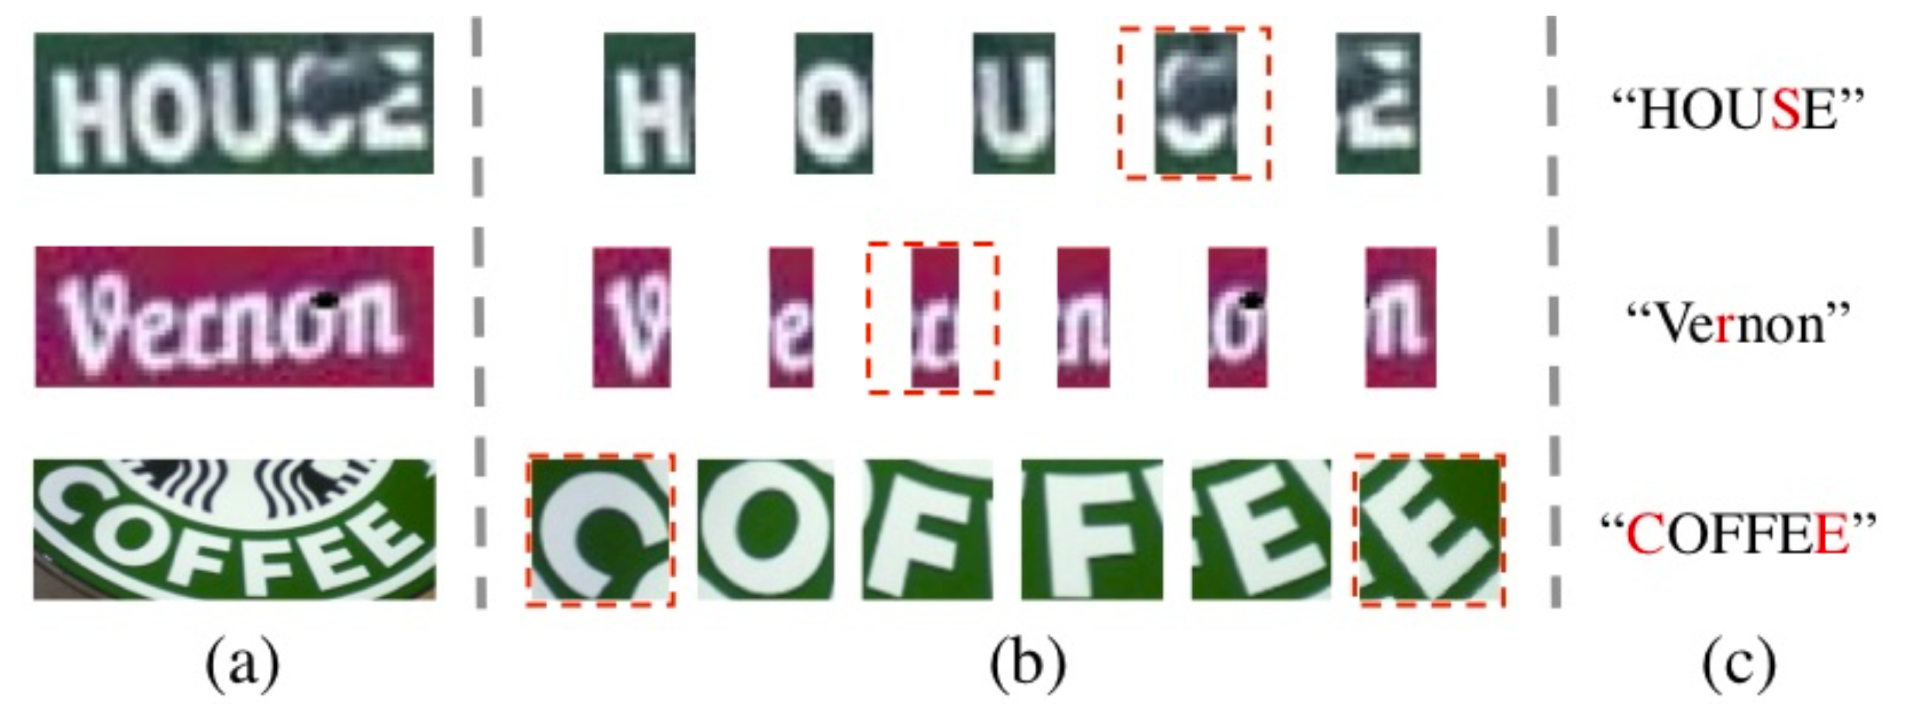
\includegraphics[width=.98\textwidth]{figure/recognition/srn_introduction.png} 
    \caption{单词中容易预测错误的字符案例:(a)表示原图;(b)表示字符,红色标注为易错字符;(c)为利用上下文语义信息预测结果。} 
    \label{srn_introduction} 
\end{figure}

\begin{figure}[H]
    \centering
    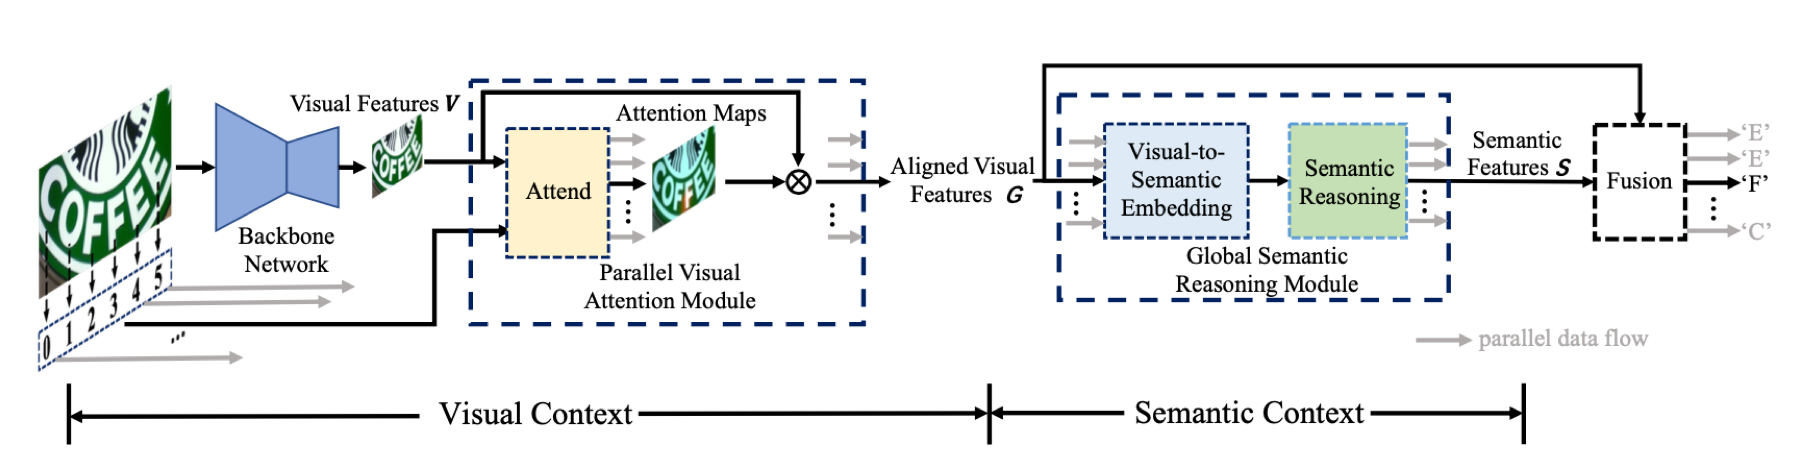
\includegraphics[width=.98\textwidth]{figure/recognition/srn_framework.png} 
    \caption{SRN网络框架图。} 
    \label{srn_framework} 
\end{figure}